% IMPI paper - IEEEtran conference mode. Every result number is a macro from numbers.tex (scripts/build_macros.py)
% or comes from an \input table (scripts/posthoc/s08_paper_assets.py). Do not type results by hand.
\RequirePackage{iftex}
\ifXeTeX
  % XeTeX (e.g. Tectonic): IEEEtran probes the Type-1 Times family 'ptm' while loading; map those probes
  % silently, then set TeX Gyre Termes (Times clone) / Cursor (Courier clone) with fontspec below.
  \DeclareFontFamily{TU}{ptm}{}
  \DeclareFontShape{TU}{ptm}{m}{n}{<->ssub * lmr/m/n}{}
  \DeclareFontShape{TU}{ptm}{m}{it}{<->ssub * lmr/m/it}{}
  \DeclareFontShape{TU}{ptm}{bx}{n}{<->ssub * lmr/bx/n}{}
  \DeclareFontShape{TU}{ptm}{bx}{it}{<->ssub * lmr/bx/it}{}
  \DeclareFontShape{TU}{ptm}{b}{n}{<->ssub * lmr/bx/n}{}
  \DeclareFontShape{TU}{ptm}{b}{it}{<->ssub * lmr/bx/it}{}
\fi
\documentclass[conference]{IEEEtran}
\IEEEoverridecommandlockouts
\usepackage{cite}
\usepackage{amsmath,amssymb}
\usepackage{graphicx}
\usepackage{booktabs}
\usepackage{array}
\usepackage{url}
\ifXeTeX
  \usepackage{newtxmath}
  \usepackage{fontspec}
  \setmainfont{texgyretermes}[Extension=.otf, UprightFont=*-regular, BoldFont=*-bold,
    ItalicFont=*-italic, BoldItalicFont=*-bolditalic]
  \setmonofont{texgyrecursor}[Extension=.otf, UprightFont=*-regular, BoldFont=*-bold,
    ItalicFont=*-italic, BoldItalicFont=*-bolditalic]
\else
  % pdfLaTeX (e.g. Overleaf): IEEEtran's standard Times setup
  \usepackage[T1]{fontenc}
  \usepackage{newtxtext,newtxmath}
\fi
\usepackage{textcomp}
% generated by scripts/build_macros.py from result JSON - do not edit by hand
\newcommand{\NTradingDays}{3,161}
\newcommand{\DataStart}{2014-01-01}
\newcommand{\DataEnd}{2026-10-09}
\newcommand{\NEquityRowsM}{5.84}
\newcommand{\NEquityRows}{5,836,673}
\newcommand{\NSymbols}{3,748}
\newcommand{\NFOUnderlyings}{354}
\newcommand{\FOPerDayMin}{134}
\newcommand{\FOPerDayMax}{227}
\newcommand{\NStaleFiles}{92}
\newcommand{\NDelivOverlapDates}{12}
\newcommand{\NDelivOverlapMismatch}{0}
\newcommand{\NFOOverlapDays}{5}
\newcommand{\NAdjust}{1,442}
\newcommand{\NAdjustNSE}{841}
\newcommand{\NAdjustGap}{468}
\newcommand{\NAdjustDemerger}{133}
\newcommand{\NGOneChecks}{57}
\newcommand{\GOneMaxDiff}{0}
\newcommand{\NFeatures}{80}
\newcommand{\NBroadTrain}{2,102}
\newcommand{\NBroadVal}{978}
\newcommand{\NBroadTest}{1,796}
\newcommand{\NBroadTotal}{4,876}
\newcommand{\SuccBroad}{0.262}
\newcommand{\NAllTrain}{5,075}
\newcommand{\NAllVal}{1,979}
\newcommand{\NAllTest}{4,273}
\newcommand{\NAllTotal}{11,327}
\newcommand{\SuccAll}{0.249}
\newcommand{\NStrictTrain}{38}
\newcommand{\NStrictVal}{15}
\newcommand{\NStrictTest}{29}
\newcommand{\NStrictTotal}{82}
\newcommand{\SuccStrict}{0.241}
\newcommand{\TvHOneExp}{27.3}
\newcommand{\TvHOneRest}{26.2}
\newcommand{\TvHOneDiff}{+1.0}
\newcommand{\TvHOneP}{0.513}
\newcommand{\TvHOneQ}{0.94}
\newcommand{\TvHTwoExp}{26.7}
\newcommand{\TvHTwoRest}{26.8}
\newcommand{\TvHTwoP}{0.936}
\newcommand{\TvHThreeExp}{1.03}
\newcommand{\TvHThreeRest}{1.07}
\newcommand{\TvHThreeP}{0.801}
\newcommand{\ValAUCxgb}{0.492}
\newcommand{\ValAUCrf}{0.487}
\newcommand{\ValAUClogit}{0.528}
\newcommand{\ValAUCcomp}{0.506}
\newcommand{\XgbTrees}{14}
\newcommand{\XgbDepth}{2}
\newcommand{\HOneExp}{24.8}
\newcommand{\HOneRest}{24.9}
\newcommand{\HOneDiff}{\ensuremath{-}0.04}
\newcommand{\HOneP}{0.987}
\newcommand{\HOneQ}{0.987}
\newcommand{\HTwoExp}{23.5}
\newcommand{\HTwoRest}{26.3}
\newcommand{\HTwoDiff}{\ensuremath{-}2.8}
\newcommand{\HTwoP}{0.171}
\newcommand{\HTwoQ}{0.286}
\newcommand{\HThreeExp}{1.01}
\newcommand{\HThreeRest}{0.88}
\newcommand{\HThreeP}{0.384}
\newcommand{\HThreeQ}{0.480}
\newcommand{\AUCxgb}{0.460}
\newcommand{\AUCrf}{0.466}
\newcommand{\AUClogit}{0.468}
\newcommand{\AUCcomp}{0.526}
\newcommand{\HFourDiff}{\ensuremath{-}0.066}
\newcommand{\HFourSE}{0.023}
\newcommand{\HFourP}{0.005}
\newcommand{\HFourQ}{0.024}
\newcommand{\TopMLPrec}{22.4}
\newcommand{\TopCompPrec}{31.0}
\newcommand{\TopMLN}{165}
\newcommand{\TopP}{0.108}
\newcommand{\TopSpread}{\ensuremath{-}0.26}
\newcommand{\TopSpreadLo}{\ensuremath{-}1.29}
\newcommand{\TopSpreadHi}{+0.64}
\newcommand{\BrierRaw}{0.250}
\newcommand{\BrierCal}{0.195}
\newcommand{\WFAUC}{0.502}
\newcommand{\WFMonths}{46}
\newcommand{\NPHTwoDiff}{\ensuremath{-}5.6}
\newcommand{\NPHTwoP}{0.026}
\newcommand{\NPHTwoQ}{0.128}
\newcommand{\NPHFourDiff}{\ensuremath{-}0.039}
\newcommand{\NPHFourP}{0.141}
\newcommand{\BHm}{5}
\newcommand{\BaseRateTest}{0.248}
\newcommand{\TTwoDiff}{+0.8}
\newcommand{\TTwoP}{0.586}
\newcommand{\PowRuleN}{144}
\newcommand{\PowRuleDiff}{\ensuremath{-}0.2}
\newcommand{\PowRuleP}{0.978}
\newcommand{\LadBaseN}{159,972}
\newcommand{\LadBase}{26.7}
\newcommand{\LadAll}{24.9}
\newcommand{\LadAllDiff}{\ensuremath{-}1.9}
\newcommand{\LadAllP}{0.005}
\newcommand{\LadBroad}{24.8}
\newcommand{\LadComp}{41.4}
\newcommand{\LadCompN}{29}
\newcommand{\CagrAll}{\ensuremath{-}26.8}
\newcommand{\TradesAll}{2,736}
\newcommand{\MaxDDAll}{\ensuremath{-}68.6}
\newcommand{\CagrBroad}{\ensuremath{-}12.6}
\newcommand{\TradesBroad}{1,599}
\newcommand{\MaxDDBroad}{\ensuremath{-}39.2}
\newcommand{\CagrComp}{+6.0}
\newcommand{\TradesComp}{29}
\newcommand{\MaxDDComp}{\ensuremath{-}1.0}
\newcommand{\CagrML}{+4.3}
\newcommand{\TradesML}{157}
\newcommand{\MaxDDML}{\ensuremath{-}2.3}
\newcommand{\CagrNifty}{+9.7}
\newcommand{\SPAp}{0.77}
\newcommand{\RCp}{0.89}
\newcommand{\DSRtrials}{89}
\newcommand{\TrialsBefore}{67}
\newcommand{\TrialsTestRun}{22}
\newcommand{\TrialsThroughPSix}{89}
\newcommand{\PreregCommit}{15103f1}
\newcommand{\PreregTime}{08:54}
\newcommand{\LockHead}{ea49def}
\newcommand{\LockStart}{09:23}
\newcommand{\LockCommit}{359bcc7}
\newcommand{\LockCommitTime}{09:30}
\newcommand{\TostHOneLo}{\ensuremath{-}3.7}
\newcommand{\TostHOneHi}{+3.6}
\newcommand{\TostHOneP}{0.19}
\newcommand{\TostHTwoLo}{\ensuremath{-}6.2}
\newcommand{\TostHTwoHi}{+0.6}
\newcommand{\TostHTwoP}{0.65}
\newcommand{\TostNPHOneLo}{\ensuremath{-}1.9}
\newcommand{\TostNPHOneHi}{+7.2}
\newcommand{\TostNPHOneP}{0.59}
\newcommand{\TostNPHTwoLo}{\ensuremath{-}9.8}
\newcommand{\TostNPHTwoHi}{\ensuremath{-}1.5}
\newcommand{\TostNPHTwoP}{0.93}
\newcommand{\MDEHOne}{6.26}
\newcommand{\MDEHTwo}{5.71}
\newcommand{\ExpN}{47}
\newcommand{\ExpRemoved}{331}
\newcommand{\ExpDiff}{\ensuremath{-}1.4}
\newcommand{\ExpP}{0.572}
\newcommand{\ExpPMin}{0.516}
\newcommand{\PSIpcr}{0.55}
\newcommand{\PSIclient}{0.31}
\newcommand{\PSInModerate}{7}
\newcommand{\PSInLarge}{2}
\newcommand{\BrierConstVal}{0.188}
\newcommand{\BrierConstTest}{0.187}
\newcommand{\IncompleteBroad}{4}
\newcommand{\GapEvents}{165}
\newcommand{\GapTrades}{157}
\newcommand{\GapSlotsFull}{8}
\newcommand{\RoundTrip}{0.58}
\newcommand{\RTLarge}{0.45}
\newcommand{\RTSmall}{0.75}
\newcommand{\AvgWin}{+4.74}
\newcommand{\AvgLoss}{\ensuremath{-}1.85}
\newcommand{\WinLossSpread}{6.59}
\newcommand{\BreakEven}{8.8}
\newcommand{\BEHOneDiff}{\ensuremath{-}0.0}
\newcommand{\BEHOneLo}{\ensuremath{-}4.4}
\newcommand{\BEHOneHi}{+4.3}
\newcommand{\BEHOneBLo}{\ensuremath{-}5.3}
\newcommand{\BEHOneBHi}{+4.7}
\newcommand{\BEHOneN}{1265}
\newcommand{\BEHTwoDiff}{\ensuremath{-}2.8}
\newcommand{\BEHTwoLo}{\ensuremath{-}6.8}
\newcommand{\BEHTwoHi}{+1.2}
\newcommand{\BEHTwoBLo}{\ensuremath{-}8.3}
\newcommand{\BEHTwoBHi}{+2.1}
\newcommand{\BEHTwoN}{924}
\newcommand{\BENPHOneDiff}{+2.6}
\newcommand{\BENPHOneLo}{\ensuremath{-}2.8}
\newcommand{\BENPHOneHi}{+8.1}
\newcommand{\BENPHOneBLo}{\ensuremath{-}2.8}
\newcommand{\BENPHOneBHi}{+7.9}
\newcommand{\BENPHOneN}{899}
\newcommand{\BENPHTwoDiff}{\ensuremath{-}5.6}
\newcommand{\BENPHTwoLo}{\ensuremath{-}10.6}
\newcommand{\BENPHTwoHi}{\ensuremath{-}0.7}
\newcommand{\BENPHTwoBLo}{\ensuremath{-}12.3}
\newcommand{\BENPHTwoBHi}{+0.7}
\newcommand{\BENPHTwoN}{617}
\newcommand{\BEMLDiff}{\ensuremath{-}2.7}
\newcommand{\BEMLLo}{\ensuremath{-}9.4}
\newcommand{\BEMLHi}{+4.1}
\newcommand{\BEMLBLo}{\ensuremath{-}13.8}
\newcommand{\BEMLBHi}{+7.3}
\newcommand{\BEMLN}{165}
\newcommand{\BECompTopDiff}{+7.0}
\newcommand{\BECompTopLo}{+0.6}
\newcommand{\BECompTopHi}{+13.4}
\newcommand{\BECompTopBLo}{+0.8}
\newcommand{\BECompTopBHi}{+15.0}
\newcommand{\BECompTopN}{226}
\newcommand{\BECompRuleDiff}{+16.8}
\newcommand{\BECompRuleLo}{\ensuremath{-}1.2}
\newcommand{\BECompRuleHi}{+34.9}
\newcommand{\BECompRuleBLo}{\ensuremath{-}10.0}
\newcommand{\BECompRuleBHi}{+46.3}
\newcommand{\BECompRuleN}{29}
\newcommand{\BEnBelow}{3}
\newcommand{\SpecOneN}{54}
\newcommand{\SpecOnePred}{89}
\newcommand{\SpecOneSig}{15}
\newcommand{\SpecOneSigPct}{28}
\newcommand{\SpecOneOpp}{0}
\newcommand{\SpecOneBH}{3}
\newcommand{\SpecOneMedian}{+2.36}
\newcommand{\SpecOneMax}{5.05}
\newcommand{\SpecOneCIAbove}{4}
\newcommand{\SpecOneFrozen}{\ensuremath{-}0.04}
\newcommand{\SpecOneRank}{49}
\newcommand{\SpecTwoN}{18}
\newcommand{\SpecTwoPred}{94}
\newcommand{\SpecTwoSig}{3}
\newcommand{\SpecTwoSigPct}{17}
\newcommand{\SpecTwoOpp}{0}
\newcommand{\SpecTwoBH}{0}
\newcommand{\SpecTwoMedian}{\ensuremath{-}2.24}
\newcommand{\SpecTwoMax}{4.44}
\newcommand{\SpecTwoCIAbove}{0}
\newcommand{\SpecTwoFrozen}{\ensuremath{-}2.81}
\newcommand{\SpecTwoRank}{6}
\newcommand{\BFOneUni}{17.88}
\newcommand{\BFNPOneUni}{9.31}
\newcommand{\BFOneSkep}{2.27}
\newcommand{\BFNPOneSkep}{1.27}
\newcommand{\BFOneLogDef}{8.41}
\newcommand{\BFNPOneLogDef}{4.49}
\newcommand{\BFOneLogSkep}{2.32}
\newcommand{\BFNPOneLogSkep}{1.43}
\newcommand{\BFTwoUni}{7.65}
\newcommand{\BFNPTwoUni}{1.31}
\newcommand{\BFTwoSkep}{1.05}
\newcommand{\BFNPTwoSkep}{0.23}
\newcommand{\BFTwoLogDef}{3.63}
\newcommand{\BFNPTwoLogDef}{0.67}
\newcommand{\BFTwoLogSkep}{1.13}
\newcommand{\BFNPTwoLogSkep}{0.30}
\newcommand{\EOneBOne}{+0.008}
\newcommand{\EOneBOneLo}{\ensuremath{-}0.237}
\newcommand{\EOneBOneHi}{+0.254}
\newcommand{\EOneBOneP}{0.946}
\newcommand{\EOneBTwo}{\ensuremath{-}0.225}
\newcommand{\EOneBTwoLo}{\ensuremath{-}0.592}
\newcommand{\EOneBTwoHi}{+0.142}
\newcommand{\EOneBTwoP}{0.229}
\newcommand{\EOneBThree}{+0.246}
\newcommand{\EOneBThreeLo}{\ensuremath{-}0.130}
\newcommand{\EOneBThreeHi}{+0.622}
\newcommand{\EOneBThreeP}{0.200}
\newcommand{\ETwoBOne}{\ensuremath{-}0.129}
\newcommand{\ETwoBOneLo}{\ensuremath{-}0.361}
\newcommand{\ETwoBOneHi}{+0.102}
\newcommand{\ETwoBOneP}{0.273}
\newcommand{\ETwoBTwo}{+0.185}
\newcommand{\ETwoBTwoLo}{+0.006}
\newcommand{\ETwoBTwoHi}{+0.364}
\newcommand{\ETwoBTwoP}{0.043}
\newcommand{\ETwoBThree}{\ensuremath{-}0.186}
\newcommand{\ETwoBThreeLo}{\ensuremath{-}0.435}
\newcommand{\ETwoBThreeHi}{+0.063}
\newcommand{\ETwoBThreeP}{0.142}
\newcommand{\EMonthMatches}{exactly}
\newcommand{\FYears}{12}
\newcommand{\FYearsSig}{0}
\newcommand{\FFirstYear}{2015}
\newcommand{\FLastYear}{2026}
\newcommand{\GTieShareLoss}{0.12}
\newcommand{\GTieExplained}{0.1}
\newcommand{\GDayOneBO}{15.0}
\newcommand{\GDayOneNB}{10.3}
\newcommand{\GRangeBO}{1.07}
\newcommand{\GRangeNB}{0.95}
\newcommand{\GGapBO}{0.11}
\newcommand{\GGapNB}{0.05}
\newcommand{\GATRBO}{2.55}
\newcommand{\GATRNB}{2.68}
\newcommand{\GAgree}{100.0}
\newcommand{\placeboDraws}{1,000}
\newcommand{\placeboActual}{\ensuremath{-}0.04}
\newcommand{\placeboMean}{+1.65}
\newcommand{\placeboSD}{1.97}
\newcommand{\placeboP}{0.795}
\newcommand{\placeboPct}{20}
\newcommand{\PSevenActual}{+1.05}
\newcommand{\PSevenDraws}{20}
\newcommand{\PSevenGE}{0}

\raggedbottom

\begin{document}

\title{Do Delivery and Futures-Positioning Footprints Predict Breakout Success? A Pre-Registered Test on Survivorship-Free NSE Data}

\author{
\IEEEauthorblockN{Fazil T}
\IEEEauthorblockA{Dept.\ of CSE (AI \& ML)\\Hindustan Institute of\\Technology and Science\\Chennai, India}
\and
\IEEEauthorblockN{Faizur Rahman S}
\IEEEauthorblockA{Dept.\ of CSE (AI \& ML)\\Hindustan Institute of\\Technology and Science\\Chennai, India}
\and
\IEEEauthorblockN{Suhail Ahmed S}
\IEEEauthorblockA{Dept.\ of CSE (AI \& ML)\\Hindustan Institute of\\Technology and Science\\Chennai, India}
\and
\IEEEauthorblockN{Jeyavim Sherin R C}
\IEEEauthorblockA{Dept.\ of CSE (AI \& ML)\\Hindustan Institute of\\Technology and Science\\Chennai, India}
}

\maketitle

\begin{abstract}
Indian traders read two daily, publicly available footprints as signs that informed money is active in a
stock: the delivery percentage, the share of traded quantity settled into demat accounts, and changes in
futures positioning. We ask whether these footprints, alone or together, predict which price breakouts
succeed. We rebuild a survivorship-free, corporate-action-adjusted panel of official National Stock
Exchange (NSE) files (\DataStart{} to \DataEnd{}, \NSymbols{} symbols), define breakout events, label each
with a triple barrier (+2/$-$1 ATR, 10 days), and test four hypotheses that were committed to version
control before any confirmatory analysis; the test set (January 2023 to \DataEnd) was evaluated once. None of the
hypotheses is supported. Delivery expansion changes test-set success by \HOneDiff{} percentage points (pp)
($p=\HOneP$); rising price with falling open interest points the predicted way (\HTwoDiff{} pp) but does not
survive false-discovery control ($q=\HTwoQ$); XGBoost ranks breakouts worse than a fixed-weight composite
(AUC \AUCxgb{} vs.\ \AUCcomp). The design could detect effects of about \MDEHOne{} pp, so smaller effects
cannot be ruled out. In post-hoc analyses on the full test set, the 95\% confidence intervals for H1 and H2
stay within the \BreakEven{} pp change in success rate needed to pay one round trip of Indian trading costs;
after costs no strategy beats the Nifty~500. We report the null result in full, with its audit trail.
\end{abstract}

\begin{IEEEkeywords}
Pre-registration, delivery percentage, open interest, institutional positioning, breakout, multiple testing,
backtest overfitting, XGBoost, National Stock Exchange of India
\end{IEEEkeywords}

% =====================================================================================================
\section{Introduction}
Theories of informed trading predict that trades by better-informed investors leave traces in prices and
order flow \cite{kyle1985,glosten1985}, and measures of the probability of informed trading and of
``flow toxicity'' have been built on intraday trade data \cite{easley1996,easley2012}. Those theories are our
motivation only: this paper does \emph{not} measure order-flow toxicity, and it uses no intraday data. Our
setting is the end-of-day data that NSE publishes for free. Indian market participants widely read two
such footprints as signs of informed activity. The first is the delivery percentage, the share of a day's
traded quantity that is settled into demat accounts rather than squared off within the day. The second is
futures positioning: a stock's own open interest (OI) and the market-wide long and short positions that NSE
reports for foreign institutional investors (FIIs), domestic institutions (DIIs), proprietary desks and
clients. A common belief is that a breakout carried by high delivery and supportive positioning is ``real''.

Many published trading signals are selected after many specifications have been tried, and selection
inflates backtests \cite{harvey2016,bailey2014pseudo}. We therefore built the study so that a negative answer
would be credible \cite{nosek2018}. We pre-registered four hypotheses on BROAD compression breakouts:
\begin{itemize}
\item \textbf{H1}: breakouts whose base shows delivery expansion succeed more often;
\item \textbf{H2}: breakouts where price rises while the stock's futures OI falls succeed less often;
\item \textbf{H3}: breakouts in a regime of FII net selling and DII net buying show a better gain-to-loss ratio;
\item \textbf{H4}: XGBoost on the same features beats a fixed-weight composite in AUC and top-decile precision.
\end{itemize}

The contributions are four. (i) IMPI, a pipeline that rebuilds a survivorship-free, point-in-time NSE panel
from official archives, including delivery data before October 2019 that NSE no longer serves in its current
format. (ii) A pre-registered design whose test set was opened once, with a disclosed timeline
(Section~\ref{sec:prereg}). (iii) A complete confirmatory null result, reported with its minimum detectable
effect and with a cost-based reading of what effect sizes would matter. (iv) A clearly separated set of
post-hoc robustness analyses (placebo, cost break-even, specification curve, Bayes factors, cluster-robust
inference) that show how far the null extends and where it does not.

% =====================================================================================================
\section{Related Work}
\subsection{Informed-Flow Theory}
In Kyle's model an insider trades gradually so that prices absorb information over time \cite{kyle1985};
in Glosten and Milgrom's model the spread compensates the market maker for adverse selection
\cite{glosten1985}. Easley et al.\ estimate the probability of informed trading from trade imbalances
\cite{easley1996}, and VPIN extends the idea to volume-synchronised, high-frequency data \cite{easley2012}.
All of these need trade-level data; we borrow only the intuition that informed activity may leave a
daily footprint.

\subsection{Institutional Flow in India}
Thapa et al.\ use transaction-level records to show that FIIs sold Indian stocks quickly after an unexpected
tax-policy announcement and traded in the direction of past returns \cite{thapa2026}. Firm-level daily FII
flows are not public. NSE publishes stock-level OI and only market-wide participant positions, so in this study
participant positioning can act only as a market regime, not as a stock-level signal. Among the papers we
reviewed we found no peer-reviewed test of NSE delivery percentage or futures positioning as a predictor of
breakout success.

\subsection{Machine Learning for Stock Prediction}
Several studies report gains from nonlinear models over linear baselines for return prediction
\cite{fieberg2023,azevedo2023,lu2025,farimani2024,gonzaleznunez2025}, while Lu et al.\ note that models
are rarely tested on firms they have not seen \cite{lu2024}. Explainability methods, chiefly SHAP for tree
ensembles \cite{lundberg2020}, are now common in financial ML \cite{cerneviciene2024,martins2024,yeo2025}.
We use XGBoost \cite{chen2016} against a simple rule-based composite rather than a weak baseline.

\subsection{Multiple Testing and Backtest Overfitting}
Harvey, Liu and Zhu argue that factor discoveries need much higher significance thresholds once the number
of tests is counted \cite{harvey2016}. Bailey and L\'opez de Prado's deflated Sharpe ratio corrects for the
number of trials and for non-normal returns \cite{bailey2014dsr}, and backtest overfitting can make
out-of-sample results worse than chance \cite{bailey2014pseudo}. We control the false discovery rate with
Benjamini--Hochberg \cite{benjamini1995}, compare strategies with Hansen's SPA test \cite{hansen2005} and
White's Reality Check \cite{white2000}, and log every trial.

% =====================================================================================================
\section{Data and Method}
\begin{figure*}[t]
\centering
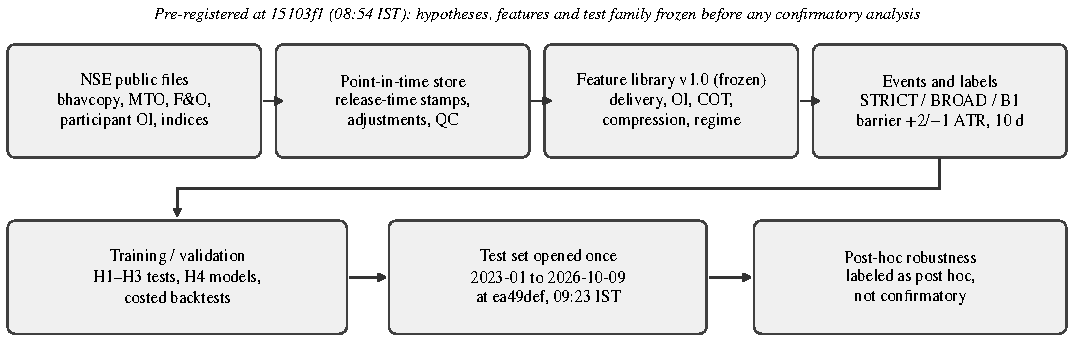
\includegraphics[width=\textwidth]{figs/fig1_pipeline.pdf}
\caption{The IMPI pipeline. Every stage reads only data published by the decision time; the hypotheses,
features and test family were frozen before any confirmatory analysis, and the test set was evaluated once.}
\label{fig:pipeline}
\end{figure*}

Fig.~\ref{fig:pipeline} shows the IMPI pipeline.

\subsection{Data}
All inputs are public NSE end-of-day files (Table~\ref{tab:dataset}): \NTradingDays{} trading days and
\NEquityRowsM{} million daily equity rows for \NSymbols{} symbols, including later-delisted stocks, so the
panel is free of survivorship bias. F\&O eligibility is taken point-in-time from each day's F\&O bhavcopy:
\NFOUnderlyings{} underlyings appear over the period, \FOPerDayMin{}--\FOPerDayMax{} on any day. Before
October 2019 delivery is rebuilt from the legacy equity bhavcopy and the MTO delivery file; on the
\NDelivOverlapDates{} dates where both formats exist the rebuilt values match the modern file with
\NDelivOverlapMismatch{} mismatches, and the two F\&O formats agree on all \NFOOverlapDays{} overlap days.
\NStaleFiles{} stale files that NSE served under holiday dates were rejected. We made \NAdjust{} split, bonus
and demerger adjustments (\NAdjustNSE{} confirmed by NSE records, \NAdjustGap{} detected from price gaps,
\NAdjustDemerger{} demergers), applied to prices, volumes and OI.

% generated by scripts/posthoc/s08_paper_assets.py from result JSON - do not edit by hand
\begin{table}[t]
\centering
\caption{Dataset summary (official NSE files)}
\label{tab:dataset}
\footnotesize
\setlength{\tabcolsep}{4pt}
\begin{tabular}{@{}>{\raggedright\arraybackslash}p{3.7cm}>{\raggedright\arraybackslash}p{4.4cm}@{}}
\toprule
\textbf{Item} & \textbf{Value} \\
\midrule
Period & 2014-01-01 to 2026-10-09 \\
Trading days & 3,161 \\
Daily equity rows & 5,836,673 \\
Symbols (incl.\ delisted) & 3,748 \\
Futures and options (F\&O) underlyings & 354 over time; 134--227 per day \\
Delivery rebuild vs.\ modern file & 0 mismatches on 12 overlap dates \\
F\&O old vs.\ new file format & 0 mismatches on 5 overlap days \\
Stale files rejected & 92 \\
Duplicate symbol-date rows & 0 \\
Delivery coverage (worst year) & 99.33\% \\
Corporate-action adjustments & 1,442 \\
\bottomrule
\end{tabular}
\par\smallskip\parbox{0.98\linewidth}{\scriptsize\raggedright Sources: results/metrics/qc\_report.json, adjustment\_qc.json, results/posthoc/paper\_facts.json.}
\end{table}


\subsection{Universe, Splits and Look-Ahead Control}
Tier~1 contains stocks in the F\&O segment on the day. A stock-day is excluded if the stock is in the F\&O
ban list, near a results date announced by $T$, priced below Rs~20, or has too short a history. Data are
split by time into training (June 2015--2020), validation (2021--2022) and test (January 2023 to
\DataEnd) periods, purging events whose label window crosses a boundary. Every file carries its publication
time; features for day $T$ use only data released by 23:59 on $T$, and trades enter at the open of $T+1$.
Recomputing features on \NGOneChecks{} truncated copies of the data changed no past value (maximum absolute
difference \GOneMaxDiff).

\subsection{Events and Label}
STRICT events are an algorithmic volatility contraction pattern \cite{minervini2013}; BROAD events are
closes above the prior 20-day high after compression (Bollinger-band-width percentile below 30 on at least 5
of the previous 10 days); B1 is every close above the prior 20-day high. BROAD is the confirmatory event set
(Table~\ref{tab:events}). Each event is labelled with a triple barrier \cite{lopezdeprado2018}: with entry $E$
at the open of $T+1$ and $A$ the 14-day ATR,
\begin{equation}
y=\begin{cases}1 & \text{if } E+2A \text{ is hit before } E-A \text{ within 10 days},\\ 0 & \text{otherwise.}\end{cases}
\end{equation}
A day that touches both barriers counts as a loss. Events whose label window is incomplete at the data end
are excluded (\IncompleteBroad{} BROAD events).

% generated by scripts/posthoc/s08_paper_assets.py from result JSON - do not edit by hand
\begin{table}[t]
\centering
\caption{Tier-1 eligible events by split (frozen at P2)}
\label{tab:events}
\footnotesize
\setlength{\tabcolsep}{4pt}
\begin{tabular}{@{}lrrrrr@{}}
\toprule
\textbf{Event set} & \textbf{Train} & \textbf{Val.} & \textbf{Test} & \textbf{Purged} & \textbf{Success} \\
\midrule
STRICT (VCP) & 38 & 15 & 29 & 1 & 0.241 \\
BROAD & 2,102 & 978 & 1,796 & 131 & 0.262 \\
B1 (20-day highs) & 5,075 & 1,979 & 4,273 & 282 & 0.249 \\
\bottomrule
\end{tabular}
\par\smallskip\parbox{0.98\linewidth}{\scriptsize\raggedright Purged = label window crosses a split boundary or is incomplete. Success = share with label$_{10}=1$ (all splits).}
\end{table}


\subsection{Features, Tests and Models}
The \NFeatures{} frozen features cover delivery (level, 20-day $z$-score, accumulation), volume and
illiquidity, compression and VCP descriptors, the stock's own OI change, commitments-of-traders style
positioning of FIIs, DIIs, Pro and Client accounts in index and stock futures, futures basis, put--call
ratio and market regime. H1 and H2 compare success rates with a two-proportion $z$-test and a calendar-month
block bootstrap; H3 compares the gain-to-loss asymmetry ratio, mean maximum favourable excursion over mean
absolute maximum adverse excursion, by block bootstrap. A logistic model with controls,
\begin{equation}
\operatorname{logit}\Pr(y=1)=\beta_0+\beta_1 D+\beta_2 P+\beta_3 (D\times P)+\gamma^{\top}x,
\label{eq:logit}
\end{equation}
estimates the interaction $\beta_3$ of the exposure $D$ with a second factor $P$ (for H1: positioning
alignment; for H2: delivery $z$-score), with controls $x$ for turnover, volatility regime, liquidity bucket
and sector. The pre-registered family has eight tests (H1--H3 on STRICT and BROAD events, H4-AUC and
H4-top-decile), controlled with Benjamini--Hochberg at $q=0.10$; by a pre-registered rule no $p$-value is
computed for a group with fewer than 30 events. For H4, XGBoost, a random forest and logistic regression
are tuned by purged 5-fold cross-validation with an embargo, calibrated by isotonic regression on validation
data, and compared with the fixed-weight composite by DeLong's test \cite{delong1988}.

\subsection{Backtest}
Signals are traded with Rs~10~lakh, at most 20 equal-weight positions, entry at the next open, exit at the
barrier, and full Indian delivery costs: securities transaction tax, exchange and SEBI fees, stamp duty, GST,
brokerage, depository charges and 5--20 basis points of slippage per side by liquidity bucket. Idle cash
earns a risk-free rate. We report CAGR against the Nifty~500, the deflated Sharpe ratio \cite{bailey2014dsr},
Hansen's SPA \cite{hansen2005} and White's Reality Check \cite{white2000}.

% =====================================================================================================
\section{Pre-Registration and Integrity}\label{sec:prereg}
The hypotheses, event definitions, test family and decision rules were committed to git in
\texttt{\PreregCommit} at \PreregTime{} IST on 10 October 2026, together with the frozen feature library.
Table~\ref{tab:timeline} gives the full timeline from git and the run logs. Three points need stating plainly.

\emph{Lock.} The single test run started at \LockStart{} IST with the repository at commit
\texttt{\LockHead}, which holds the code and the training/validation results. The run itself wrote the
lock file, which was first committed in \texttt{\LockCommit} at \LockCommitTime{} IST together with the test
results. (An earlier draft cited \texttt{\LockHead} as the lock commit.)

\emph{Trials.} Of the \TrialsThroughPSix{} rows in the results log up to the test evaluation,
\TrialsBefore{} were written before the test run started and \TrialsTestRun{} were written by the test run
itself. The deflated Sharpe ratio used all \DSRtrials, which is conservative.

\emph{Disclosure.} Data download, corporate-action fixes and quality control used the full period. For its
power calculation, the pre-registration document lists the event counts and the overall success rate of
each split, the test split included; it contains no result split by any hypothesis exposure. Our earlier
pilot study had explored July 2025 to October 2026, inside the test period, so all confirmatory results are
also reported without that window.

% generated by scripts/posthoc/s08_paper_assets.py from result JSON - do not edit by hand
\begin{table}[t]
\centering
\caption{Pre-registration timeline, 10 Oct 2026 (IST, from git and run logs)}
\label{tab:timeline}
\footnotesize
\setlength{\tabcolsep}{4pt}
\begin{tabular}{@{}ll>{\raggedright\arraybackslash}p{5.9cm}@{}}
\toprule
\textbf{Commit} & \textbf{Time} & \textbf{Event} \\
\midrule
\texttt{355cbe0} & 02:16 & IMPI P0-P2 scaffolding: config, NSE ingest, PIT store, adjustment \ldots \\
\texttt{86ddfd7} & 08:21 & Adjustment fixes on full data: downward-only gap snaps, stale ex-date \ldots \\
\texttt{b5829b2} & 08:40 & Ban list: first-day publication time = previous evening (G1 check strict) \\
-- & 08:53 & P2 writes feature freeze (features, events, labels) \\
\texttt{15103f1} & 08:54 & PRE-REGISTRATION: hypotheses H1-H4, decision rules, P2 counts/power \ldots \\
-- & 08:54 & P3 first analysis rows (train+val.) in results log \\
\texttt{ea49def} & 09:23 & P3-P5 results (train/validation): hypotheses, composite ladder/backtests \ldots \\
-- & 09:23 & P6 starts: test set opened; lock written (HEAD = ea49def) \\
\texttt{359bcc7} & 09:30 & P6: one-time test-set evaluation (lock ea49def) \\
\texttt{1fc97ae} & 12:01 & IMPI v2 (post-hoc) models, live mode with forward track record, shared day \ldots \\
\bottomrule
\end{tabular}
\par\smallskip\parbox{0.98\linewidth}{\scriptsize\raggedright 67 of the 89 results-log rows through P6 were written before the test run; the other 22 are the test run's own rows. The lock file was first committed in 359bcc7. Data download, adjustment fixes and QC (before the pre-registration) used the full period. The pre-registration itself lists test-set event counts and the overall test success rate (power table), but no result split by any hypothesis exposure.}
\end{table}


% =====================================================================================================
\section{Results}
\subsection{Exploratory Results (Training and Validation)}
On training and validation data, BROAD breakouts with delivery expansion succeeded \TvHOneExp\% of the time
against \TvHOneRest\% without (\TvHOneDiff{} pp, $p=\TvHOneP$, $q=\TvHOneQ$). H2 rates were \TvHTwoExp\% and
\TvHTwoRest\% ($p=\TvHTwoP$) and H3 asymmetry ratios \TvHThreeExp{} and \TvHThreeRest{} ($p=\TvHThreeP$).
On validation, XGBoost reached an AUC of \ValAUCxgb, the random forest \ValAUCrf, logistic regression
\ValAUClogit{} and the composite \ValAUCcomp; XGBoost stopped early at \XgbTrees{} trees of depth \XgbDepth.

\subsection{Confirmatory Results (Test Set, Run Once)}
Table~\ref{tab:confirm} gives the pre-registered family. All three STRICT groups have fewer than 30 events
per arm, so the pre-registered guard withholds their $p$-values; the Benjamini--Hochberg procedure therefore
runs over $m=\BHm$ finite $p$-values, not eight. No hypothesis is supported.

\textbf{H1.} Delivery expansion made no difference: \HOneExp\% against \HOneRest\% (\HOneDiff{} pp,
$p=\HOneP$). \textbf{H2.} Breakouts with rising price and falling OI succeeded \HTwoExp\% against
\HTwoRest\% (\HTwoDiff{} pp, $p=\HTwoP$, $q=\HTwoQ$); without the pilot window the gap is \NPHTwoDiff{} pp
($p=\NPHTwoP$) but $q=\NPHTwoQ$ remains above 0.10. \textbf{H3.} The asymmetry ratio was \HThreeExp{} in the
FII-selling, DII-buying regime against \HThreeRest{} otherwise ($p=\HThreeP$). \textbf{H4.} XGBoost ranked
breakouts worse than the composite: AUC \AUCxgb{} against \AUCcomp{} (difference \HFourDiff, SE \HFourSE,
DeLong $p=\HFourP$, $q=\HFourQ$). This is the only rejection in the family and it is in the wrong direction.
The random forest (\AUCrf) and logistic regression (\AUClogit) were no better, and a walk-forward version
with \WFMonths{} monthly refits reached \WFAUC. Top-decile precision was \TopMLPrec\% for XGBoost
($n=\TopMLN$) against \TopCompPrec\% for the composite ($p=\TopP$).

Why did the model fail? The features it relied on most are market-wide positioning variables, whose
distribution shifted between training and test: the population stability index is \PSIpcr{} for the
put--call ratio and \PSIclient{} for client index-futures positioning, both above the 0.25 level usually
read as a large shift (post-hoc). Isotonic calibration lowered the Brier score \cite{brier1950} from
\BrierRaw{} to \BrierCal, but a constant forecast at the validation base rate scores \BrierConstVal{} on the
test set, so the calibrated model is worse than predicting no skill at all.

\textbf{Power.} With the test-set group sizes, the pre-registered design has 80\% power at $\alpha=0.05$ to
detect a difference of \MDEHOne{} pp for H1 and \MDEHTwo{} pp for H2. Effects smaller than this cannot be
ruled out by the confirmatory tests. In particular, the data do not establish equivalence within $\pm$2 pp:
a two-one-sided-tests check \cite{lakens2017} gives 90\% intervals of [\TostHOneLo, \TostHOneHi] pp for H1
($p_{\mathrm{TOST}}=\TostHOneP$) and [\TostHTwoLo, \TostHTwoHi] pp for H2 ($p_{\mathrm{TOST}}=\TostHTwoP$),
both failing (post-hoc).

% generated by scripts/posthoc/s08_paper_assets.py from result JSON - do not edit by hand
\begin{table}[t]
\centering
\caption{Pre-registered confirmatory family on the test set (BH, $q=0.10$, $m=5$)}
\label{tab:confirm}
\footnotesize
\setlength{\tabcolsep}{4pt}
\begin{tabular}{llrrrcr}
\toprule
\textbf{Test} & \textbf{Set} & $n$ & \textbf{Diff.} & $p$ & \textbf{Rank} & $q$ \\
\midrule
\multicolumn{7}{l}{\textit{Full test set (2023-01-01 to 2026-10-09)}} \\
H1 & STRICT & 29 & +12.99 & n$<$30 (0.484) & -- & -- \\
H2 & STRICT & 28 & +11.28 & n$<$30 (0.468) & -- & -- \\
H3 & STRICT & 29 & \ensuremath{-}0.077 & n$<$30 (0.942) & -- & -- \\
H1 & BROAD & 1,796 & \ensuremath{-}0.04 & 0.987 & 5 & 0.987 \\
H2 & BROAD & 1,776 & \ensuremath{-}2.81 & 0.171 & 3 & 0.286 \\
H3 & BROAD & 1,769 & +0.124 & 0.384 & 4 & 0.480 \\
H4 auc & BROAD & 1,796 & \ensuremath{-}0.066 & 0.005 & 1 & 0.024 \\
H4 top decile & BROAD & 1,796 & \ensuremath{-}8.55 & 0.108 & 2 & 0.270 \\
\midrule
\multicolumn{7}{l}{\textit{Without pilot window (before 2025-07-28)}} \\
H1 & STRICT & 23 & +13.33 & n$<$30 (0.567) & -- & -- \\
H2 & STRICT & 22 & +13.33 & n$<$30 (0.484) & -- & -- \\
H3 & STRICT & 23 & +0.622 & n$<$30 (0.478) & -- & -- \\
H1 & BROAD & 1,236 & +2.62 & 0.352 & 4 & 0.440 \\
H2 & BROAD & 1,221 & \ensuremath{-}5.65 & 0.026 & 1 & 0.128 \\
H3 & BROAD & 1,213 & \ensuremath{-}0.083 & 0.759 & 5 & 0.759 \\
H4 auc & BROAD & 1,236 & \ensuremath{-}0.039 & 0.141 & 2 & 0.351 \\
H4 top decile & BROAD & 1,236 & \ensuremath{-}9.37 & 0.258 & 3 & 0.430 \\
\bottomrule
\end{tabular}
\par\smallskip\parbox{0.98\linewidth}{\scriptsize\raggedright PRE-REGISTERED. Diff.\ in pp for H1, H2 and H4-top-decile; H3 = difference in gain-to-loss asymmetry ratio; H4-AUC = AUC difference XGBoost $-$ composite. STRICT tests have fewer than 30 events per arm, so the pre-registered guard withholds their $p$ (unguarded value in brackets, not used); BH therefore runs over $m=5$ finite $p$-values. The only rejection (H4-AUC) is in the wrong direction: XGBoost ranks worse than the composite. No hypothesis is supported.}
\end{table}


\subsection{Post-hoc Analyses}
\emph{Everything in this subsection was designed after the test set was opened and is exploratory.}
Table~\ref{tab:audit} lists the audit checks and Table~\ref{tab:robust} the robustness results.

\textbf{Cost break-even.} One round trip in the backtest cost model costs \RoundTrip\% on average (\RTLarge\%
for large to \RTSmall\% for small stocks). A successful BROAD trade returned \AvgWin\% gross and a failed one
\AvgLoss\%, a spread of \WinLossSpread{} pp, so a change of $d$ in success rate is worth $d$ times this spread
per trade and pays one round trip only when $d\ge\BreakEven$ pp. The 95\% intervals for H1 (\BEHOneLo{} to
\BEHOneHi{} pp; month-block \BEHOneBLo{} to \BEHOneBHi), H1 without the pilot (\BENPHOneLo{} to \BENPHOneHi),
and H2 (\BEHTwoLo{} to \BEHTwoHi) all lie inside $\pm$\BreakEven{} pp. For H2 without the pilot window the
interval (\BENPHTwoLo{} to \BENPHTwoHi; month-block \BENPHTwoBLo{} to \BENPHTwoBHi) reaches beyond the
break-even in the predicted direction, so an economically relevant effect cannot be excluded there. Two
non-hypothesis contrasts against the remaining BROAD events: the ML top decile, \BEMLDiff{} pp
(\BEMLLo{} to \BEMLHi), and the composite top decile, \BECompTopDiff{} pp (\BECompTopLo{} to \BECompTopHi;
$n=\BECompTopN$), whose interval excludes zero but includes the break-even.

\textbf{Placebo.} Shuffling delivery across the test-event stocks within each day and recomputing the
delivery features \placeboDraws{} times gives a placebo H1 effect of \placeboMean{} pp on average
(SD \placeboSD); the actual effect of \placeboActual{} pp lies at the \placeboPct{}th percentile (one-sided
empirical $p=\placeboP$; Fig.~\ref{fig:placebo}). The earlier \PSevenDraws-draw placebo on training and
validation data had found an effect of \PSevenActual{} pp, with \PSevenGE\% of draws at least as large.
On the test set the placebo draws are on average larger than the actual effect, so randomly reassigning
delivery among stocks on the same day does at least as well as the stock's own delivery: the test data give no
sign of stock-specific delivery information, and the earlier training-period reading is not reproduced.

\textbf{Specification curve.} We re-ran H1 over 3 barrier settings, 3 horizons, 3 delivery-expansion
thresholds and 2 event sets (\SpecOneN{} specifications) and H2 over the same grid without the threshold
(\SpecTwoN) \cite{simonsohn2020}. The frozen specification is the pre-registered one; the curve is
post-hoc. For H1, \SpecOnePred\% of specifications point in the predicted direction, \SpecOneSig{}
(\SpecOneSigPct\%) are significant at 5\% (\SpecOneOpp{} in the opposite direction), and \SpecOneBH{} survive
Benjamini--Hochberg at $q=0.10$ within the curve. The median effect is \SpecOneMedian{} pp and the largest
\SpecOneMax{} pp, below the \BreakEven{} pp break-even, although the 95\% interval of \SpecOneCIAbove{}
specifications reaches it. The frozen specification (\SpecOneFrozen{} pp) ranks \SpecOneRank{} of
\SpecOneN{} in the predicted direction: stricter delivery thresholds and wider barriers give larger effects.
For H2, \SpecTwoPred\% point in the predicted direction, \SpecTwoSig{} (\SpecTwoSigPct\%) are significant,
\SpecTwoBH{} survive Benjamini--Hochberg, the median is \SpecTwoMedian{} pp, the largest in the predicted
(negative) direction \SpecTwoMax{} pp,
and the frozen specification (\SpecTwoFrozen{} pp) ranks \SpecTwoRank{} of \SpecTwoN. The specifications
share events and are not independent tests (Fig.~\ref{fig:spec}).

\textbf{Bayes factors.} For the two-binomial comparison \cite{kass1995}, BF$_{01}$ (evidence for no
difference) for H1 is \BFOneUni{} under uniform priors and \BFOneLogDef{} under a unit-normal prior on the
log odds ratio \cite{gronau2021}, but only \BFOneSkep{} and \BFOneLogSkep{} under skeptical priors that let
the alternative predict effects of a few pp. For H2 the values are \BFTwoUni, \BFTwoLogDef, \BFTwoSkep{} and
\BFTwoLogSkep; without the pilot window the skeptical-prior values for H2 fall to \BFNPTwoSkep{} and
\BFNPTwoLogSkep, which favour a difference. The evidence for a null is therefore strong only under wide
priors \cite{leewagenmakers2013}.

\textbf{Cluster-robust model.} Re-estimating \eqref{eq:logit} on the test set with standard errors clustered
two-way by date and stock \cite{cameron2011} gives, for H1, $\beta_1=\EOneBOne$ [\EOneBOneLo, \EOneBOneHi],
$\beta_2=\EOneBTwo$ [\EOneBTwoLo, \EOneBTwoHi] and the interaction $\beta_3=\EOneBThree$
[\EOneBThreeLo, \EOneBThreeHi] ($p=\EOneBThreeP$). For H2, $\beta_1=\ETwoBOne$ ($p=\ETwoBOneP$),
$\beta_2=\ETwoBTwo$ [\ETwoBTwoLo, \ETwoBTwoHi] ($p=\ETwoBTwoP$) and $\beta_3=\ETwoBThree$
[\ETwoBThreeLo, \ETwoBThreeHi] ($p=\ETwoBThreeP$). Month-clustered errors reproduce the locked test values
\EMonthMatches.

\textbf{Other checks.} Excluding events in the 5 sessions before each of the \ExpN{} monthly F\&O expiries
leaves H1 at \ExpDiff{} pp ($p=\ExpP$). By calendar year, \FYearsSig{} of the \FYears{} yearly BROAD H1
estimates from \FFirstYear{} to \FLastYear{} are significant at 5\% (Fig.~\ref{fig:forest}).
Breakouts succeed less often than all eligible stock-days (\LadAll\% against \LadBase\%); same-day barrier
ties are only \GTieShareLoss\% of breakout losses and explain \GTieExplained\% of the gap. Instead, breakouts
are stopped out on their first day more often (\GDayOneBO\% against \GDayOneNB\%) and have wider next-day
ranges (\GRangeBO{} against \GRangeNB{} ATR) with larger opening gaps (\GGapBO{} against \GGapNB{} ATR).
The re-labelling used here reproduces the frozen labels in \GAgree\% of cases. Of the \GapEvents{} ML
top-decile events, \GapTrades{} were traded; the other \GapSlotsFull{} arrived when all 20 slots were full.

% generated by scripts/posthoc/s08_paper_assets.py from result JSON - do not edit by hand
\begin{table}[t]
\centering
\caption{Supplementary audit of the locked test evaluation}
\label{tab:audit}
\footnotesize
\setlength{\tabcolsep}{4pt}
\begin{tabular}{@{}>{\raggedright\arraybackslash}p{3.0cm}l>{\raggedright\arraybackslash}p{3.4cm}@{}}
\toprule
\textbf{Check} & \textbf{Label} & \textbf{Result} \\
\midrule
MDE, H1 / H2 (80\%, $\alpha$=.05) & PRE-REG. & 6.26 / 5.71 pp \\
Cost break-even $d^*$ & POST-HOC & 0.58\% / 6.59 pp = 8.8 pp \\
TOST $\pm$2 pp, H1 (full) & POST-HOC & 90\% CI [\ensuremath{-}3.7, +3.6], $p$=0.19 \\
TOST $\pm$2 pp, H2 (full) & POST-HOC & 90\% CI [\ensuremath{-}6.2, +0.6], $p$=0.65 \\
H1 excl.\ 5 sessions pre-expiry & POST-HOC & \ensuremath{-}1.4 pp, $p$=0.57 (331 removed) \\
PSI $>$0.25 among top-10 SHAP & POST-HOC & client\_fut\_idx\_cot 0.31, log\_pcr\_oi 0.55 \\
Brier: constant / calibrated XGB & POST-HOC & 0.1879 / 0.1953 \\
Incomplete labels (last 10 days) & PRE-REG.\ rule & 4 BROAD events excluded \\
ML top decile: events vs trades & PRE-REG.\ rule & 165 vs 157 (slots full) \\
\bottomrule
\end{tabular}
\par\smallskip\parbox{0.98\linewidth}{\scriptsize\raggedright POST-HOC rows were designed after the test set was opened (10 Oct 2026, 09:23 IST). Brier constant uses the validation base rate (no test information).}
\end{table}

% generated by scripts/posthoc/s08_paper_assets.py from result JSON - do not edit by hand
\begin{table*}[t]
\centering
\caption{Post-hoc robustness on the test set}
\label{tab:robust}
\footnotesize
\setlength{\tabcolsep}{4pt}
\begin{tabular}{llll}
\toprule
\textbf{Hyp.} & \textbf{Spec./prior/term} & \textbf{Value} & \textbf{Reading (full test)} \\
\midrule
\multicolumn{4}{l}{\textit{Specification curve (barrier $\times$ horizon $\times$ threshold $\times$ event set)}} \\
H1 & 54 specs & 15 sig.\ (28\%), 0 opposite & median +2.36 pp; frozen \ensuremath{-}0.04 pp \\
H2 & 18 specs & 3 sig.\ (17\%), 0 opposite & median \ensuremath{-}2.24 pp; frozen \ensuremath{-}2.81 pp \\
\midrule
\multicolumn{4}{l}{\textit{Bayes factor BF$_{01}$ (BROAD, full test / without pilot)}} \\
H1 & Beta(1,1) & 17.88 / 9.31 & strong evidence for H0 (no difference) \\
H1 & skeptical Beta & 2.27 / 1.27 & anecdotal evidence for H0 (no difference) \\
H1 & logOR$\sim$N(0,1) & 8.41 / 4.49 & moderate evidence for H0 (no difference) \\
H1 & logOR$\sim$N(0,0.25$^2$) & 2.32 / 1.43 & anecdotal evidence for H0 (no difference) \\
H2 & Beta(1,1) & 7.65 / 1.31 & moderate evidence for H0 (no difference) \\
H2 & skeptical Beta & 1.05 / 0.23 & anecdotal evidence for H0 (no difference) \\
H2 & logOR$\sim$N(0,1) & 3.63 / 0.67 & moderate evidence for H0 (no difference) \\
H2 & logOR$\sim$N(0,0.25$^2$) & 1.13 / 0.30 & anecdotal evidence for H0 (no difference) \\
\midrule
\multicolumn{4}{l}{\textit{Logit model, Eq.~(\ref{eq:logit}), on the test set, BROAD, two-way (date $\times$ symbol) clustered SE}} \\
H1 & $\beta_1$ deliv\_exp & +0.008 [\ensuremath{-}0.237, +0.254] & $p$=0.946 \\
H1 & $\beta_2$ pos & \ensuremath{-}0.225 [\ensuremath{-}0.592, +0.142] & $p$=0.229 \\
H1 & $\beta_3$ deliv\_exp:pos & +0.246 [\ensuremath{-}0.130, +0.622] & $p$=0.200 \\
H2 & $\beta_1$ div & \ensuremath{-}0.129 [\ensuremath{-}0.361, +0.102] & $p$=0.273 \\
H2 & $\beta_2$ dz & +0.185 [+0.006, +0.364] & $p$=0.043 \\
H2 & $\beta_3$ div:dz & \ensuremath{-}0.186 [\ensuremath{-}0.435, +0.063] & $p$=0.142 \\
\bottomrule
\end{tabular}
\par\smallskip\parbox{0.95\linewidth}{\scriptsize\raggedright ALL POST-HOC. Specs overlap and are not corrected for multiplicity. BF$_{01}>1$ favours no difference; it shrinks towards 1 under skeptical priors that let the alternative predict small effects. Month-clustered SEs reproduce the locked P6 values exactly; STRICT logits are not estimable ($n=28$, separation).}
\end{table*}


\begin{figure*}[t]
\centering
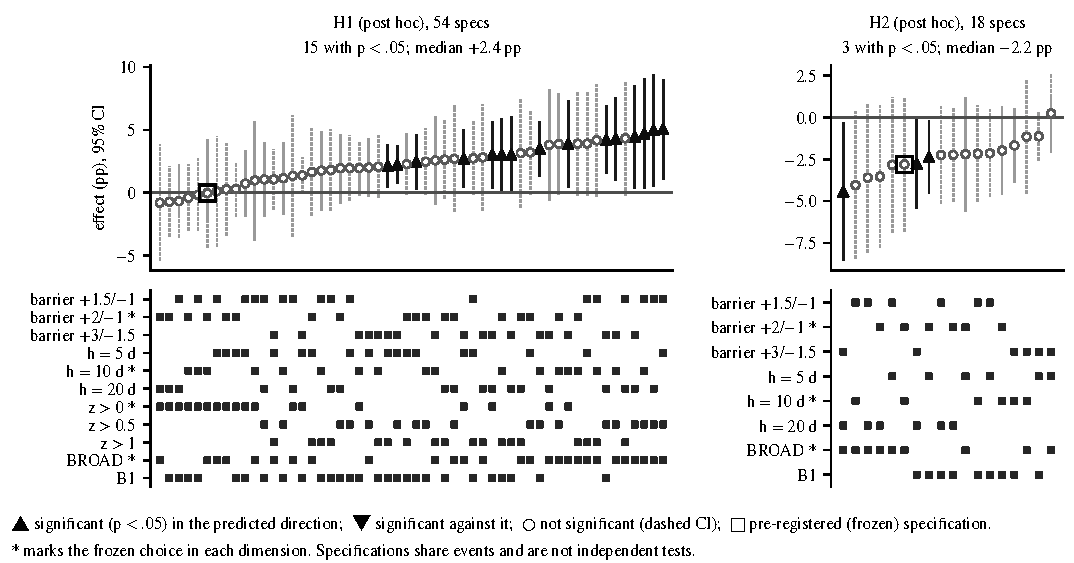
\includegraphics[width=\textwidth]{figs/fig_spec_curve.pdf}
\caption{Post-hoc specification curve on the test set. Top: success-rate difference with 95\% CI for each
specification, sorted; the outlined dot is the pre-registered specification. Bottom: the choices behind each
specification.}
\label{fig:spec}
\end{figure*}

\begin{figure}[t]
\centering
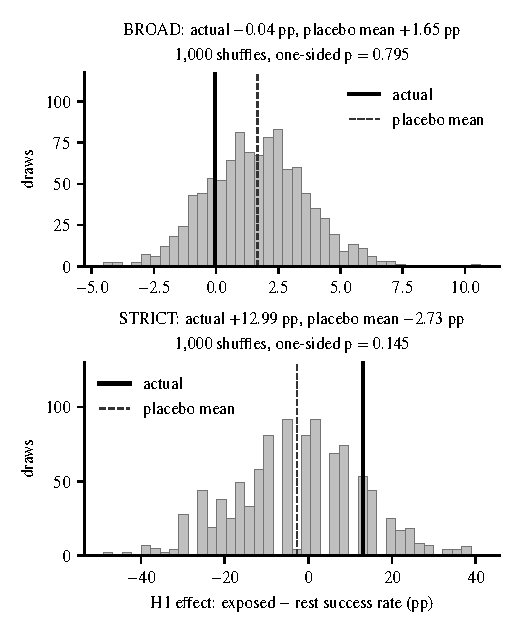
\includegraphics[width=\columnwidth]{figs/fig_placebo_hist.pdf}
\caption{Post-hoc placebo on the test set: H1 effect under within-day shuffles of delivery across stocks,
with the actual effect marked.}
\label{fig:placebo}
\end{figure}

\begin{figure}[t]
\centering
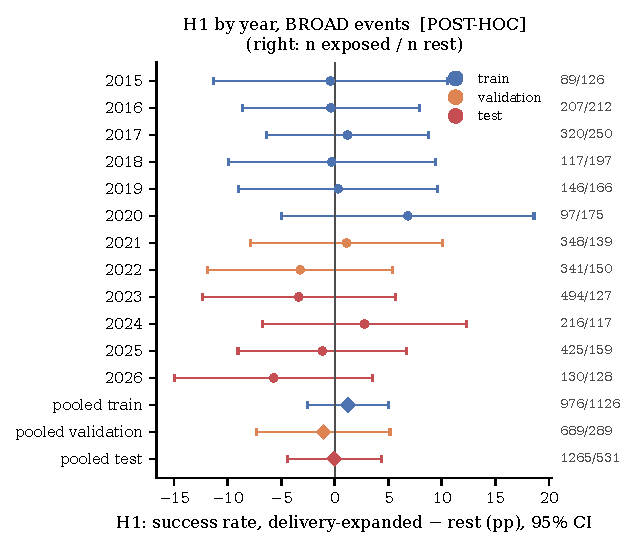
\includegraphics[width=\columnwidth]{figs/fig_h1_forest.pdf}
\caption{Post-hoc H1 effect by calendar year with 95\% CIs, coloured by split.}
\label{fig:forest}
\end{figure}

\subsection{Benchmark Ladder and Backtests (Pre-Registered)}
Across the \LadBaseN{} eligible stock-days of the test period, \LadBase\% met the success condition;
breakouts did worse at \LadAll\% (\LadAllDiff{} pp, $p=\LadAllP$), and adding compression (BROAD,
\LadBroad\%) did not help (Fig.~\ref{fig:ladder}). Stocks with a composite score of at least 1 succeeded
\LadComp\% of the time, but only \LadCompN{} events qualified, below the pre-registered minimum of 30.
After all costs (Table~\ref{tab:backtests}, Fig.~\ref{fig:cagr}), trading every breakout returned \CagrAll\%
a year and BROAD breakouts \CagrBroad\%; the composite (\TradesComp{} trades) and the ML top decile
(\TradesML{} trades) returned \CagrComp\% and \CagrML\%, all below the Nifty~500's \CagrNifty\%. Neither SPA
($p=\SPAp$) nor the Reality Check ($p=\RCp$) finds a strategy that beats the benchmark, and every deflated
Sharpe ratio is zero.

\begin{figure}[t]
\centering
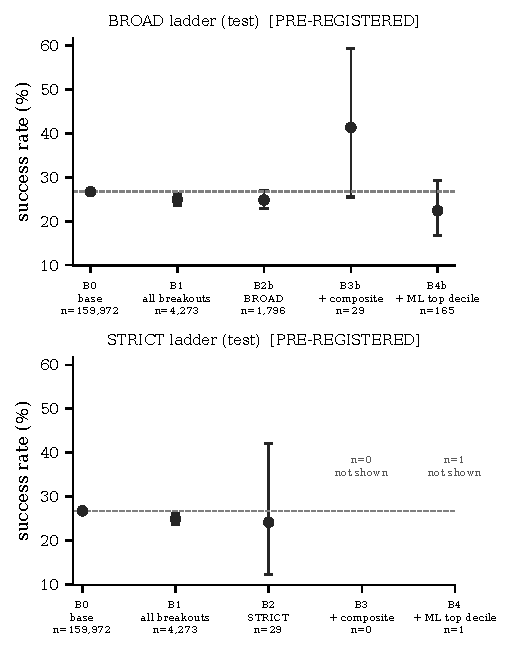
\includegraphics[width=\columnwidth]{figs/fig_ladder.pdf}
\caption{Ten-day success rate of each rung of the pre-registered benchmark ladder in the test period, with
Wilson 95\% intervals. The dashed line is the base rate over all eligible stock-days.}
\label{fig:ladder}
\end{figure}

% generated by scripts/posthoc/s08_paper_assets.py from result JSON - do not edit by hand
\begin{table*}[t]
\centering
\caption{Costed test-set backtests (2023-01 to 2026-10)}
\label{tab:backtests}
\footnotesize
\setlength{\tabcolsep}{4pt}
\begin{tabular}{lrrrrrrl}
\toprule
\textbf{Strategy} & \textbf{Trades} & \textbf{CAGR} & \textbf{Sharpe} & \textbf{MaxDD} & \textbf{Hit\%} & \textbf{PF} &  \\
\midrule
B1 all breakouts & 2,736 & \ensuremath{-}26.8 & \ensuremath{-}4.02 & \ensuremath{-}68.6 & 31.5 & 0.59 & ok \\
B2 STRICT & 29 & +5.7 & \ensuremath{-}0.47 & \ensuremath{-}0.5 & 34.5 & 0.72 & n$<$30 \\
B4 STRICT ML top decile & 1 & -- & -- & -- & 0.0 & 0.00 & n$<$30 \\
B2b BROAD & 1,599 & \ensuremath{-}12.6 & \ensuremath{-}3.25 & \ensuremath{-}39.2 & 32.1 & 0.60 & ok \\
B3b BROAD composite & 29 & +6.0 & \ensuremath{-}0.01 & \ensuremath{-}1.0 & 41.4 & 1.04 & n$<$30 \\
B4b BROAD ML top decile & 157 & +4.3 & \ensuremath{-}0.85 & \ensuremath{-}2.3 & 33.1 & 0.64 & ok \\
\midrule
Nifty 500 (benchmark) & -- & +9.7 & 0.32 & \ensuremath{-}18.8 & -- & -- &  \\
\bottomrule
\end{tabular}
\par\smallskip\parbox{0.95\linewidth}{\scriptsize\raggedright PRE-REGISTERED (P6, run once). Full Indian costs and slippage; max.\ 20 positions. Hansen SPA $p$=0.77, White RC $p$=0.89; deflated Sharpe $\approx 0$ for all (N = 89 results-log rows at the time of the run, of which 67 were logged before the test run started).}
\end{table*}


\begin{figure}[t]
\centering
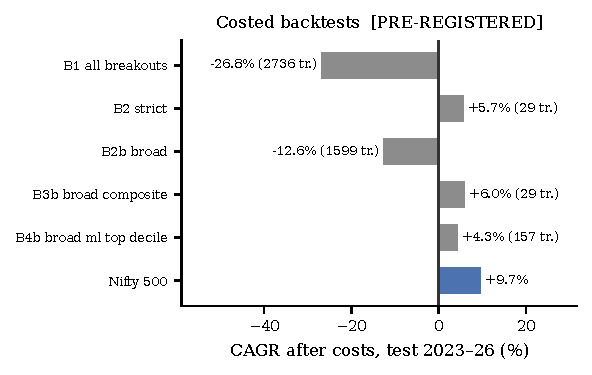
\includegraphics[width=\columnwidth]{figs/fig_cagr.pdf}
\caption{Test-period CAGR after Indian costs.}
\label{fig:cagr}
\end{figure}

% =====================================================================================================
\section{Discussion}
The pre-registered answer is no: in this design, delivery expansion, OI divergence and the FII/DII regime
do not change breakout success detectably, and a gradient-boosted model does worse than a fixed composite.
The null is informative about large effects but not about small ones: the design's detectable effect is
about \MDEHOne{} pp, the data do not establish equivalence within $\pm$2 pp, and Bayes factors favour the
null strongly only under wide priors. What the post-hoc analyses add is an economic reading: for the
pre-registered effects on the full test set, even the favourable ends of the intervals are below the
\BreakEven{} pp change in success rate that one round trip of Indian costs requires. The specification
curve qualifies this. The pre-registered specification is among the weakest on the curve, and stricter
delivery thresholds or wider barriers give positive H1 effects of a few pp, consistent with delivery carrying
information about the size of subsequent moves rather than their direction. These effects are post-hoc,
not independent of one another, mostly do not survive multiple-testing control within the curve, and remain
below the cost break-even; they are leads for a new pre-registered test, not findings. The ML failure is
largely a story of non-stationarity: the model leaned on market-wide positioning variables whose
distribution shifted between training and test.

% =====================================================================================================
\section{Limitations}
Participant positions are published only as market-wide totals, so they act as a regime variable rather than
a stock-level signal; there is no public daily FII/DII cash-flow series, and futures positions may be hedges.
The ``Client'' category mixes retail and high-net-worth accounts. STRICT events are too rare for
confirmatory inference. The sample spans structural breaks (T+1 settlement in 2023, F\&O reforms in
2024--2025). The pre-registration followed data preparation on the full period and disclosed test-set event
counts and base rates. Part of the test period had been explored by our pilot study. All trials were logged,
but logging cannot remove every researcher choice. The post-hoc analyses are many and were chosen after the
confirmatory result was known.

% =====================================================================================================
\section{Conclusion and Future Work}
Using a survivorship-free NSE panel, hypotheses fixed in advance and a test set opened once, we find no
support for the belief that delivery and futures-positioning footprints predict breakout success, and no
strategy that beats the Nifty~500 after costs. Effects smaller than the design's detectable effect remain
possible, but on the full test set they are smaller than what Indian trading costs require. Three leads from
exploration, each needing its own pre-registered test on data collected after October 2026, are:
(1) whether FIIs follow price in stock futures, with index returns preceding their stock-futures positioning;
(2) whether FII positioning in index futures precedes index returns; and (3) whether stricter delivery
thresholds predict the size of breakout moves, as the specification curve suggests. Beyond these, we plan a
market-level regime-transition model that uses participant positioning to forecast changes in volatility
regime, pre-registered and evaluated only on post-October-2026 data. Nothing in this paper is investment
advice.

% =====================================================================================================
\section*{Data and Code Availability}
All inputs are public NSE end-of-day files; they are not redistributed but are re-downloaded by the pipeline.
Code, configuration, the locked study results, the post-hoc results, the generator of every table, figure
and number in this paper, and the SHA-256 checksums of the locked files are in the project repository
(\texttt{impi/}; see \texttt{README.md} and \texttt{DATA\_AVAILABILITY.md}).

\section*{Acknowledgment}
The authors used Claude (Anthropic) via Claude Code to write and debug portions of the IMPI pipeline code,
run the post-hoc audit and robustness scripts, generate the \LaTeX{} tables and figures from the logged
results, and draft and edit text in all sections. The research question, hypotheses, pre-registration, data
sources and all interpretive decisions were made by the authors, who reviewed and verified all AI-generated
code, text and figures and take full responsibility for the content of this paper.

\bibliographystyle{IEEEtran}
\bibliography{refs}

\end{document}
